\chapter{Methodology and System Design}
The project was executed following a structured methodology, from data sourcing to final deployment. The overall system architecture is shown in Figure \ref{fig:architecture}.

\vspace{0.5cm}
\begin{figure}[H]
    \centering
    \begin{tikzpicture}[node distance=2cm]
        % Nodes
        \node (data) [process, text width=5cm] {1. Data Preparation\\(Roboflow Datasets Merged)};
        \node (train) [process, below of=data, text width=5cm] {2. Model Training\\(YOLOv8n on RunPod Server)};
        \node (export) [process, below of=train, text width=5cm] {3. Model Export \& Quantization\\(best.pt -> best\_float16.tflite)};
        \node (deploy) [startstop, below of=export, text width=5cm] {4. Deployment \& Inference\\(Raspberry Pi 3B+)};
        
        % Arrows
        \draw [arrow] (data) -- (train);
        \draw [arrow] (train) -- (export);
        \draw [arrow] (export) -- (deploy);
    \end{tikzpicture}
    \caption{System Architecture Diagram.}
    \label{fig:architecture}
\end{figure}

\section{Data Collection and Preparation}
High-quality data is the foundation of any successful deep learning model. This project utilized two datasets sourced from Roboflow.
\begin{enumerate}
    \item \textbf{Motorbike Detection Dataset:} Provided by user \texttt{cdio-zmfmj}.
    \item \textbf{Helmet \& License Plate Detection Dataset:} Also from \texttt{cdio-zmfmj}.
\end{enumerate}
These datasets were downloaded programmatically and merged to create a unified dataset with four classes: \texttt{helmet}, \texttt{no-helmet}, \texttt{motorbike}, and \texttt{license-plate}. Figure \ref{fig:training_batch} shows an example batch of images from the training set with their ground-truth labels.

\begin{figure}[H]
    \centering
    % NOTE: Make sure 'train_batch0.jpg' is in the same folder as this .tex file
    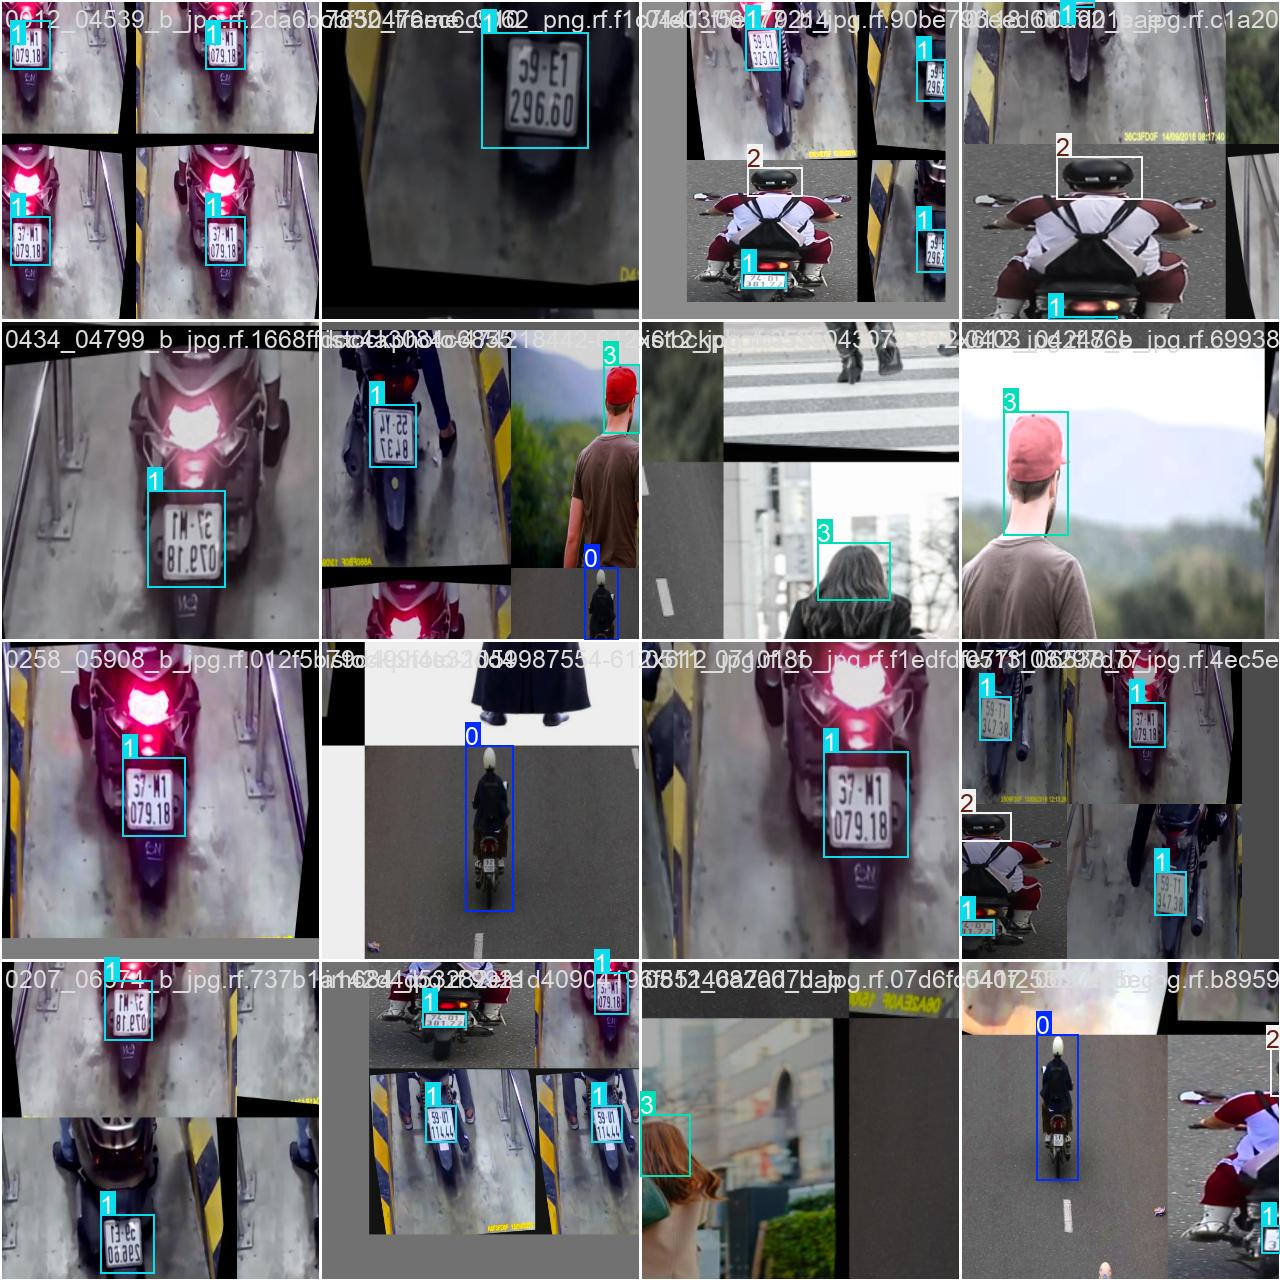
\includegraphics[width=0.8\textwidth]{../runs/detect/helmet_detection/train_batch0.jpg}
    \caption{Example of a training batch with ground-truth labels.}
    \label{fig:training_batch}
\end{figure}

\section{Model Training}
\subsection{Choice of Model and Environment}
The \texttt{YOLOv8n} model was selected due to its optimal trade-off between speed and accuracy for edge devices. Training was conducted on a RunPod cloud server equipped with a high-performance GPU to significantly reduce training time.

\subsection{Training Process}
Key training parameters were set as follows:
\begin{itemize}
    \item \textbf{Epochs:} 100
    \item \textbf{Patience:} 5 (for early stopping)
    \item \textbf{Image Size:} 320x320 pixels
    \item \textbf{Batch Size:} 16
\end{itemize}

\section{Model Conversion and Deployment}
\subsection{TFLite Conversion}
Upon completion of training, the best-performing model checkpoint (\texttt{best.pt}) was automatically converted to the TensorFlow Lite format. The \texttt{best\_float16.tflite} model was chosen for deployment.

\subsection{Raspberry Pi Setup}
The target hardware was a Raspberry Pi 3B+. The setup process involved:
\begin{enumerate}
    \item Flashing a microSD card with the Raspberry Pi OS.
    \item Installing \texttt{opencv-python-headless} and \texttt{tflite-runtime}.
    \item Transferring the model, class list, and inference script to the device.
\end{enumerate}
